\hypertarget{a00806}{}\section{M\+I\+DI}
\label{a00806}\index{MIDI@{MIDI}}
How to route and process M\+I\+DI in A\+AX plug-\/ins. 

\hypertarget{a00806_additionalFeatures_MIDI_Overview}{}\subsection{Midi Overview}\label{a00806_additionalFeatures_MIDI_Overview}
Direct\+Midi is Avid\textquotesingle{}s protocol for communication of M\+I\+DI and other timing-\/critical plug-\/in information. It is a cross-\/platform solution to tightly integrate the host application, audio engine, and plug-\/ins.\hypertarget{a00806_additionalFeatures_MIDI_NodeTypes}{}\subsection{M\+I\+D\+I node types}\label{a00806_additionalFeatures_MIDI_NodeTypes}
There are four kinds of nodes an A\+AX plug-\/in can create. See \mbox{\hyperlink{a00491_a5e1dffce35d05990dbbad651702678e4}{A\+A\+X\+\_\+\+E\+M\+I\+D\+I\+Node\+Type}} for additional details about these node types\+: \begin{DoxyItemize}
\item \mbox{\hyperlink{a00491_a5e1dffce35d05990dbbad651702678e4ae57de2b04978fe2e75f5bdeb034bda44}{A\+A\+X\+\_\+e\+M\+I\+D\+I\+Node\+Type\+\_\+\+Local\+Input}} \item \mbox{\hyperlink{a00491_a5e1dffce35d05990dbbad651702678e4acc1b5f2109c508b20a65b5e0fdcd643f}{A\+A\+X\+\_\+e\+M\+I\+D\+I\+Node\+Type\+\_\+\+Local\+Output}} \item \mbox{\hyperlink{a00491_a5e1dffce35d05990dbbad651702678e4a2be91828f8c1dac20ab5dff136fc1fce}{A\+A\+X\+\_\+e\+M\+I\+D\+I\+Node\+Type\+\_\+\+Global}} \item \mbox{\hyperlink{a00491_a5e1dffce35d05990dbbad651702678e4ac2ff856aec0724907dfd95b8e3ccbc20}{A\+A\+X\+\_\+e\+M\+I\+D\+I\+Node\+Type\+\_\+\+Transport}}\end{DoxyItemize}
\hypertarget{a00806_additionalFeatures_MIDI_AddingMIDI}{}\subsection{Adding M\+I\+D\+I functionality to a plug-\/in}\label{a00806_additionalFeatures_MIDI_AddingMIDI}
Plug-\/in may access M\+I\+DI data in its algorithm or data model. If plug-\/in needs M\+I\+DI in both places or just in the algorithm, it should add a M\+I\+DI node to the algorithm context, i.\+e. call \mbox{\hyperlink{a01781_a6284dda9ccca898e33075de29dad4e39}{A\+A\+X\+\_\+\+I\+Component\+Descriptor\+::\+Add\+M\+I\+D\+I\+Node()}} with the appropriate node type.


\begin{DoxyCode}{0}
\DoxyCodeLine{\textcolor{comment}{//==============================================================================}}
\DoxyCodeLine{\textcolor{comment}{// Algorithm context definitions}}
\DoxyCodeLine{\textcolor{comment}{//==============================================================================}}
\DoxyCodeLine{}
\DoxyCodeLine{\textcolor{comment}{// Context structure}}
\DoxyCodeLine{\textcolor{keyword}{struct }SMy\_Alg\_Context}
\DoxyCodeLine{\{}
\DoxyCodeLine{    [...]}
\DoxyCodeLine{    \mbox{\hyperlink{a01845}{AAX\_IMIDINode}}  * mMIDIInNodeP;         \textcolor{comment}{// Local input MIDI node pointer}}
\DoxyCodeLine{    \mbox{\hyperlink{a01845}{AAX\_IMIDINode}}  * mMIDINodeOutP;        \textcolor{comment}{// Local output MIDI node pointer}}
\DoxyCodeLine{    \mbox{\hyperlink{a01845}{AAX\_IMIDINode}}  * mMIDINodeTransportP;  \textcolor{comment}{// Transport node }}
\DoxyCodeLine{    [...]}
\DoxyCodeLine{\};}
\DoxyCodeLine{}
\DoxyCodeLine{\textcolor{keyword}{enum} EDemoMIDI\_Alg\_PortID}
\DoxyCodeLine{\{}
\DoxyCodeLine{    [...]}
\DoxyCodeLine{    \textcolor{comment}{//}}
\DoxyCodeLine{    \textcolor{comment}{// Add the MIDI node as a physical address within the context field}}
\DoxyCodeLine{    ,eAlgPortID\_MIDINodeIn          = \mbox{\hyperlink{a00392_acf807247ecd6e5899dc9dc31644e9a1d}{AAX\_FIELD\_INDEX}} (SDemoMIDI\_Alg\_Context, mMIDINodeP)}
\DoxyCodeLine{    ,eAlgPortID\_MIDINodeOut         = \mbox{\hyperlink{a00392_acf807247ecd6e5899dc9dc31644e9a1d}{AAX\_FIELD\_INDEX}} (SDemoMIDI\_Alg\_Context, mMIDINodeOutP)}
\DoxyCodeLine{    ,eAlgPortID\_MIDINodeTransport   = \mbox{\hyperlink{a00392_acf807247ecd6e5899dc9dc31644e9a1d}{AAX\_FIELD\_INDEX}} (SDemoMIDI\_Alg\_Context, mMIDINodeTransportP)}
\DoxyCodeLine{    [...]}
\DoxyCodeLine{\};}
\end{DoxyCode}



\begin{DoxyCode}{0}
\DoxyCodeLine{\textcolor{comment}{// ***************************************************************************}}
\DoxyCodeLine{\textcolor{comment}{// ROUTINE: DescribeAlgorithmComponent}}
\DoxyCodeLine{\textcolor{comment}{// Algorithm component description}}
\DoxyCodeLine{\textcolor{comment}{// ***************************************************************************}}
\DoxyCodeLine{\textcolor{keyword}{static} \textcolor{keywordtype}{void} DescribeAlgorithmComponent( \mbox{\hyperlink{a01781}{AAX\_IComponentDescriptor}} * outDesc )}
\DoxyCodeLine{\{}
\DoxyCodeLine{    \mbox{\hyperlink{a00392_a4d8f69a697df7f70c3a8e9b8ee130d2f}{AAX\_Result}}                    err;}
\DoxyCodeLine{    }
\DoxyCodeLine{    [...]}
\DoxyCodeLine{    \textcolor{comment}{// Register MIDI nodes}}
\DoxyCodeLine{    err = outDesc->\mbox{\hyperlink{a01781_a6284dda9ccca898e33075de29dad4e39}{AddMIDINode}}(eAlgPortID\_MIDINodeA, \mbox{\hyperlink{a00491_a5e1dffce35d05990dbbad651702678e4ae57de2b04978fe2e75f5bdeb034bda44}{AAX\_eMIDINodeType\_LocalInput}}, \textcolor{stringliteral}{"DemoMIDI"}, 0xffff);                  \mbox{\hyperlink{a00395_a168ee44fd7a5485ab50160db36fb2988}{AAX\_ASSERT}} (err == 0);}
\DoxyCodeLine{    err = outDesc->\mbox{\hyperlink{a01781_a6284dda9ccca898e33075de29dad4e39}{AddMIDINode}}(eAlgPortID\_MIDINodeOut, \mbox{\hyperlink{a00491_a5e1dffce35d05990dbbad651702678e4acc1b5f2109c508b20a65b5e0fdcd643f}{AAX\_eMIDINodeType\_LocalOutput}}, \textcolor{stringliteral}{"DemoMIDIOut"}, 0xffff);           \mbox{\hyperlink{a00395_a168ee44fd7a5485ab50160db36fb2988}{AAX\_ASSERT}} (err == 0);}
\DoxyCodeLine{    err = outDesc->\mbox{\hyperlink{a01781_a6284dda9ccca898e33075de29dad4e39}{AddMIDINode}}(eAlgPortID\_MIDINodeTransport, \mbox{\hyperlink{a00491_a5e1dffce35d05990dbbad651702678e4ac2ff856aec0724907dfd95b8e3ccbc20}{AAX\_eMIDINodeType\_Transport}}, \textcolor{stringliteral}{"DemoMIDITrnsprt"}, 0xffff); \mbox{\hyperlink{a00395_a168ee44fd7a5485ab50160db36fb2988}{AAX\_ASSERT}} (err == 0);}
\DoxyCodeLine{    [...]}
\DoxyCodeLine{\}}
\end{DoxyCode}


If M\+I\+DI data is needed in the plug-\/in\textquotesingle{}s data model only, plug-\/in should describe M\+I\+DI node with \mbox{\hyperlink{a01813_aa7709de005e0256feb522758ccc5b582}{A\+A\+X\+\_\+\+I\+Effect\+Descriptor\+::\+Add\+Control\+M\+I\+D\+I\+Node()}}.


\begin{DoxyCode}{0}
\DoxyCodeLine{\textcolor{comment}{// ***************************************************************************}}
\DoxyCodeLine{\textcolor{comment}{// ROUTINE: GetPlugInDescription}}
\DoxyCodeLine{\textcolor{comment}{// ***************************************************************************}}
\DoxyCodeLine{\textcolor{keyword}{static} \mbox{\hyperlink{a00392_a4d8f69a697df7f70c3a8e9b8ee130d2f}{AAX\_Result}} GetPlugInDescription( \mbox{\hyperlink{a01813}{AAX\_IEffectDescriptor}} * outDescriptor )}
\DoxyCodeLine{\{}
\DoxyCodeLine{    \mbox{\hyperlink{a00392_a4d8f69a697df7f70c3a8e9b8ee130d2f}{AAX\_Result}}                    err;}
\DoxyCodeLine{    }
\DoxyCodeLine{    [...]}
\DoxyCodeLine{    \textcolor{comment}{// Register MIDI nodes}}
\DoxyCodeLine{    err = outDesc->AddControlMIDINode(\textcolor{stringliteral}{'linp'}, \mbox{\hyperlink{a00491_a5e1dffce35d05990dbbad651702678e4ae57de2b04978fe2e75f5bdeb034bda44}{AAX\_eMIDINodeType\_LocalInput}}, \textcolor{stringliteral}{"DemoMIDI"}, 0xffff);        \mbox{\hyperlink{a00395_a168ee44fd7a5485ab50160db36fb2988}{AAX\_ASSERT}} (err == 0);}
\DoxyCodeLine{    err = outDesc-> AddControlMIDINode(\textcolor{stringliteral}{'lout'}, \mbox{\hyperlink{a00491_a5e1dffce35d05990dbbad651702678e4acc1b5f2109c508b20a65b5e0fdcd643f}{AAX\_eMIDINodeType\_LocalOutput}}, \textcolor{stringliteral}{"DemoMIDIOut"}, 0xffff);  \mbox{\hyperlink{a00395_a168ee44fd7a5485ab50160db36fb2988}{AAX\_ASSERT}} (err == 0);}
\DoxyCodeLine{    err = outDesc-> AddControlMIDINode(\textcolor{stringliteral}{'tran'}, \mbox{\hyperlink{a00491_a5e1dffce35d05990dbbad651702678e4ac2ff856aec0724907dfd95b8e3ccbc20}{AAX\_eMIDINodeType\_Transport}}, \textcolor{stringliteral}{"DemoMIDITrnsprt"}, 0xffff);  \mbox{\hyperlink{a00395_a168ee44fd7a5485ab50160db36fb2988}{AAX\_ASSERT}} (err == 0);}
\DoxyCodeLine{    [...]}
\DoxyCodeLine{}
\DoxyCodeLine{    \textcolor{keywordflow}{return} err;}
\DoxyCodeLine{\}}
\end{DoxyCode}


\begin{DoxyNote}{Note}
These two types of M\+I\+DI nodes can\textquotesingle{}t be used together in the same plug-\/in\textquotesingle{}s effect.
\end{DoxyNote}
\hypertarget{a00806_additionalFeatures_MIDI_Algorithm}{}\subsection{Using M\+I\+D\+I in a plug-\/in algorithm}\label{a00806_additionalFeatures_MIDI_Algorithm}
Like with other algorithm context ports, data in M\+I\+DI nodes is directly available in the plug-\/in\textquotesingle{}s algorithm process function. Here is an example from the Demo\+M\+I\+D\+I\+\_\+\+Note\+On sample plug-\/in\+:


\begin{DoxyCode}{0}
\DoxyCodeLine{\textcolor{keyword}{template}<\textcolor{keywordtype}{int} kNumChannelsIn, \textcolor{keywordtype}{int} kNumChannelsOut> }
\DoxyCodeLine{\textcolor{keywordtype}{void}}
\DoxyCodeLine{\mbox{\hyperlink{a00392_aaa22112139aa627574b1ef562f579d43}{AAX\_CALLBACK}}}
\DoxyCodeLine{DemoMIDI\_AlgorithmProcessFunction (}
\DoxyCodeLine{                                   SDemoMIDI\_Alg\_Context * \textcolor{keyword}{const}    inInstancesBegin [],}
\DoxyCodeLine{                                   \textcolor{keyword}{const} \textcolor{keywordtype}{void} *                 inInstancesEnd)}
\DoxyCodeLine{\{}
\DoxyCodeLine{    [...]}
\DoxyCodeLine{    \textcolor{comment}{// Setup MIDI In node pointers }}
\DoxyCodeLine{    \mbox{\hyperlink{a01845}{AAX\_IMIDINode}}* midiNodeIn = instance->mMIDINodeP;}
\DoxyCodeLine{    \mbox{\hyperlink{a01433}{AAX\_CMidiStream}}* midiBufferIn = midiNodeIn->\mbox{\hyperlink{a01845_a794f1c0d19ac6720382c23b0a4dc2b17}{GetNodeBuffer}}();}
\DoxyCodeLine{    \mbox{\hyperlink{a01429}{AAX\_CMidiPacket}}* midiBufferInPtr = midiBufferIn->\mbox{\hyperlink{a01433_a5011ea886dce57b382c23b82e56d3000}{mBuffer}};}
\DoxyCodeLine{    uint32\_t packets\_count\_in = midiBufferIn->\mbox{\hyperlink{a01433_ad93c962a8278977f2a4f07b1e7490a90}{mBufferSize}};}
\DoxyCodeLine{    }
\DoxyCodeLine{    \textcolor{comment}{// Setup MIDI Out node pointers }}
\DoxyCodeLine{    \mbox{\hyperlink{a01845}{AAX\_IMIDINode}}* midiNodeOut = instance->mMIDINodeOutP;}
\DoxyCodeLine{    \mbox{\hyperlink{a01433}{AAX\_CMidiStream}}* midiBufferOut = midiNodeOut->\mbox{\hyperlink{a01845_a794f1c0d19ac6720382c23b0a4dc2b17}{GetNodeBuffer}}();}
\DoxyCodeLine{    \mbox{\hyperlink{a01429}{AAX\_CMidiPacket}}* midiBufferOutPtr = midiBufferOut->\mbox{\hyperlink{a01433_a5011ea886dce57b382c23b82e56d3000}{mBuffer}};}
\DoxyCodeLine{    uint32\_t packets\_count\_out = midiBufferOut->\mbox{\hyperlink{a01433_ad93c962a8278977f2a4f07b1e7490a90}{mBufferSize}};}
\DoxyCodeLine{}
\DoxyCodeLine{    }
\DoxyCodeLine{    \textcolor{comment}{// Setup MIDI Transport node pointers }}
\DoxyCodeLine{    \mbox{\hyperlink{a01845}{AAX\_IMIDINode}}* midiTransport = instance->mMIDINodeTransportP;}
\DoxyCodeLine{    \mbox{\hyperlink{a01885}{AAX\_ITransport}} * transport = midiTransport->\mbox{\hyperlink{a01845_a57bd132ee74047e25298b157c0bff2f9}{GetTransport}}();}
\DoxyCodeLine{    \textcolor{keywordtype}{bool} transport\_is\_playing = \textcolor{keyword}{false};}
\DoxyCodeLine{    \textcolor{keywordflow}{if} (transport)}
\DoxyCodeLine{        transport->\mbox{\hyperlink{a01885_a8f7d5b8f65ff9dd456a395838c974715}{IsTransportPlaying}}(\&transport\_is\_playing);}
\DoxyCodeLine{    }
\DoxyCodeLine{    \textcolor{keywordflow}{if}(transport\_is\_playing)}
\DoxyCodeLine{    \{}
\DoxyCodeLine{        \textcolor{comment}{//}}
\DoxyCodeLine{        \textcolor{comment}{// While there are packets in the node}}
\DoxyCodeLine{        \textcolor{keywordflow}{while} (packets\_count\_in > 0)}
\DoxyCodeLine{        \{}
\DoxyCodeLine{            midiBufferOutPtr = midiBufferInPtr;         \textcolor{comment}{// Copy the packet from the input MIDI node }}
\DoxyCodeLine{                                        \textcolor{comment}{// to the output MIDI node}}
\DoxyCodeLine{            midiBufferOutPtr->\mbox{\hyperlink{a01429_a76df0e71968aa1416b93015ebf23ddc5}{mTimestamp}} = timeStamp;     \textcolor{comment}{// Set the MIDI time stamp}}
\DoxyCodeLine{            midiNodeOut->\mbox{\hyperlink{a01845_a5e1c5409158164f57376f908c9693a8b}{PostMIDIPacket}}(midiBufferOutPtr);    \textcolor{comment}{// Post the MIDI packet}}
\DoxyCodeLine{            midiBufferOut->\mbox{\hyperlink{a01433_ad93c962a8278977f2a4f07b1e7490a90}{mBufferSize}} = packets\_count\_in;   }
\DoxyCodeLine{                            }
\DoxyCodeLine{            midiBufferInPtr++;}
\DoxyCodeLine{            packets\_count\_in--;}
\DoxyCodeLine{        \}}
\DoxyCodeLine{    \}}
\DoxyCodeLine{    [...]}
\DoxyCodeLine{\}   }
\end{DoxyCode}


Also data from the M\+I\+DI nodes that were described with \mbox{\hyperlink{a01781_a6284dda9ccca898e33075de29dad4e39}{A\+A\+X\+\_\+\+I\+Component\+Descriptor\+::\+Add\+M\+I\+D\+I\+Node()}} can be accessed via \mbox{\hyperlink{a01481_aac6fa72278c0f46aa430cd79bdb2d767}{A\+A\+X\+\_\+\+C\+Effect\+Parameters\+::\+Update\+M\+I\+D\+I\+Nodes()}} method. This method provides an \mbox{\hyperlink{a01429}{A\+A\+X\+\_\+\+C\+Midi\+Packet}}. Because the M\+I\+DI packet structure does not identify the associated M\+I\+DI stream\textquotesingle{}s type (input, output, global, or transport) this method also provides an index into the plug-\/in\textquotesingle{}s algorithm context structure which can be used to identify the semantics of the M\+I\+DI packet.\hypertarget{a00806_additionalFeatures_MIDI_DataModel}{}\subsection{Accessing M\+I\+D\+I in the plug-\/in data model}\label{a00806_additionalFeatures_MIDI_DataModel}
A plug-\/in may access M\+I\+DI data in its data model via the \mbox{\hyperlink{a01481_aac6fa72278c0f46aa430cd79bdb2d767}{A\+A\+X\+\_\+\+C\+Effect\+Parameters\+::\+Update\+M\+I\+D\+I\+Nodes()}} or \mbox{\hyperlink{a01481_ac6720637afc7a87adfd391c4ef59126f}{A\+A\+X\+\_\+\+C\+Effect\+Parameters\+::\+Update\+Control\+M\+I\+D\+I\+Nodes()}} methods. Both of these methods provide an \mbox{\hyperlink{a01429}{A\+A\+X\+\_\+\+C\+Midi\+Packet}}. Because the M\+I\+DI packet structure does not identify the associated M\+I\+DI stream\textquotesingle{}s type (input, output, global, or transport) Update\+M\+I\+D\+I\+Nodes method also provides an index into the plug-\/in\textquotesingle{}s algorithm context structure which can be used to identify the semantics of the M\+I\+DI packet, while Update\+Control\+M\+I\+D\+I\+Nodes provides M\+I\+DI node ID for the same reason.


\begin{DoxyCode}{0}
\DoxyCodeLine{\mbox{\hyperlink{a00392_a4d8f69a697df7f70c3a8e9b8ee130d2f}{AAX\_Result}} DemoMIDI\_Parameters::UpdateMIDINodes ( \mbox{\hyperlink{a00392_ae807f8986143820cfb5d6da32165c9c7}{AAX\_CFieldIndex}} inFieldIndex,    \mbox{\hyperlink{a01429}{AAX\_CMidiPacket}}\& inPacket )}
\DoxyCodeLine{\{   }
\DoxyCodeLine{    \textcolor{keywordflow}{if} (eAlgPortID\_MIDINodeIn == inFieldIndex)}
\DoxyCodeLine{    \{}
\DoxyCodeLine{        \textcolor{keywordflow}{if} ( (inPacket.\mbox{\hyperlink{a01429_aac7229afc36006bc673eb219b18d8220}{mData}}[0] \& 0xF0) == 0x90 )}
\DoxyCodeLine{        \{}
\DoxyCodeLine{            \textcolor{keywordflow}{if} ( inPacket.\mbox{\hyperlink{a01429_aac7229afc36006bc673eb219b18d8220}{mData}}[2] == 0x00 )}
\DoxyCodeLine{            \{}
\DoxyCodeLine{                \textcolor{comment}{//  Note Off}}
\DoxyCodeLine{            \}}
\DoxyCodeLine{            \textcolor{keywordflow}{else}}
\DoxyCodeLine{            \{}
\DoxyCodeLine{                \textcolor{comment}{// Note On}}
\DoxyCodeLine{            \}}
\DoxyCodeLine{        \}}
\DoxyCodeLine{    \}}
\DoxyCodeLine{    }
\DoxyCodeLine{    \textcolor{keywordflow}{return} \mbox{\hyperlink{a00494_a5f8c7439f3a706c4f8315a9609811937aeddbd1bb67e3a66e6af54a4b4a7a57b3}{AAX\_SUCCESS}};}
\DoxyCodeLine{\}}
\end{DoxyCode}


\begin{DoxyNote}{Note}
Only one of the Update\+M\+I\+D\+I\+Nodes and Update\+Control\+M\+I\+D\+I\+Nodes can be used in the single plug-\/in\textquotesingle{}s effect at a time. If plug-\/in uses M\+I\+DI nodes described with Add\+M\+I\+D\+I\+Node function, then only Update\+M\+I\+D\+I\+Nodes method can be used to receive M\+I\+DI messages. Otherwise Update\+Control\+M\+I\+D\+I\+Nodes should be used. 
\end{DoxyNote}
Collaboration diagram for M\+I\+DI\+:
\nopagebreak
\begin{figure}[H]
\begin{center}
\leavevmode
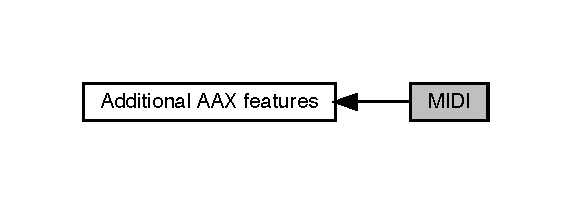
\includegraphics[width=274pt]{a00806}
\end{center}
\end{figure}
